
\section{Axis lines}
There are times where you might want an option for the axis lines
somewhere besides an outer box (the default) and through the middle.
The full range of options is \\
"axis lines = box|left|middle|center|right|none"\\
where ``"|"'' means ``or''.  

As usual, there are some other style changes that take place when you
choose one of these.  For instance
\begin{latex}
\begin{tikzpicture}
\begin{axis}["axis lines = left", xlabel={$t$}, ylabel={height}]
\addplot[only marks, domain = 0:10, thick, blue,variable=t]{-4.9*t^2+500};
\end{axis}
\end{tikzpicture}
\end{latex}
%
\begin{center}
\tikzcount
\begin{tikzpicture}
\begin{axis}[axis lines = left, xlabel={$t$}, ylabel={height}]
\addplot[only marks, domain = 0:10, thick, blue,variable=t]{-4.9*t^2+500};
\end{axis}
\end{tikzpicture}
\end{center}
Note that it wrote ``height'' sideways.  

Maybe you'd like to have a grid in this and ask students to estimate
the average velocity between two of the points
\begin{latex}
\begin{tikzpicture}
\begin{axis}[axis lines = left, "grid,"
xlabel={$t$}, ylabel={height}]
\addplot[only marks, domain = 0:10, thick, blue,variable=t]{-4.9*t^2+500};
\end{axis}
\end{tikzpicture}
\end{latex}
%
\begin{center}
\tikzcount
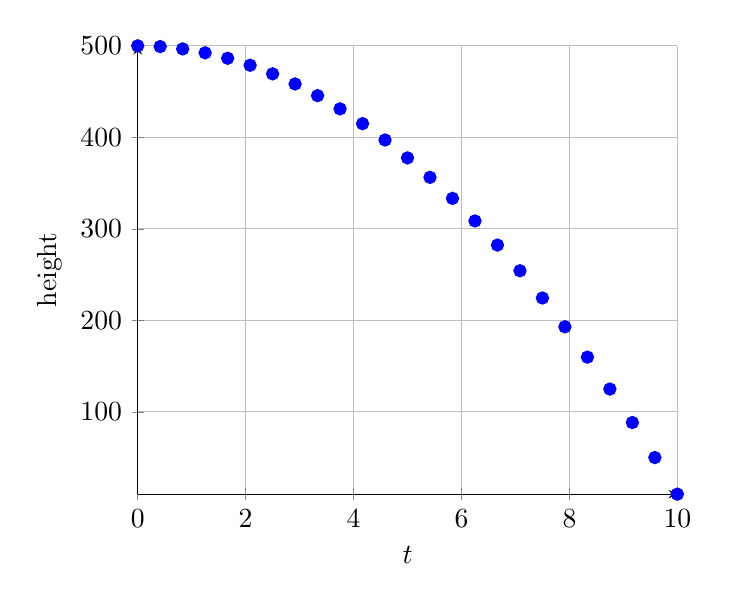
\begin{tikzpicture}
\begin{axis}[axis lines = left, grid,
xlabel={$t$}, ylabel={height}]
\addplot[only marks, domain = 0:10, thick, blue,variable=t]{-4.9*t^2+500};
\end{axis}
\end{tikzpicture}
\end{center}
Maybe you'd like a denser grid
\begin{latex}
\begin{tikzpicture}
\begin{axis}[axis lines = left, 
"grid=both," % marks both major and minor ticks
"xtick distance = 1," % x ticks every integer
"ytick distance = 50," % y ticks multiples of 50
"minor tick num=1," % one minor tick between each pair of major ticks
ymin=0,
xlabel={$t$}, ylabel={height}]
\addplot[only marks, domain = 0:10, thick, blue,variable=t]{-4.9*t^2+500};
\end{axis}
\end{tikzpicture}
\end{latex}
%
\begin{center}
\tikzcount
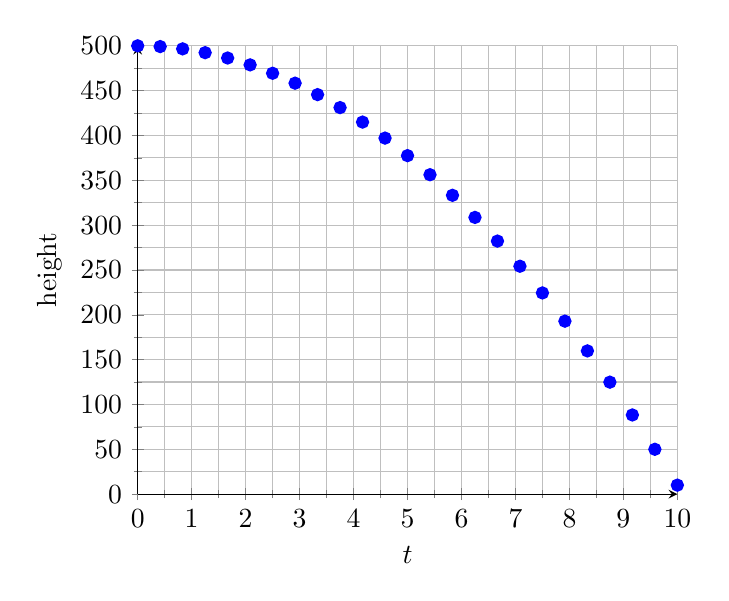
\begin{tikzpicture}
\begin{axis}[axis lines = left, 
grid=both, % marks both major and minor ticks
xtick distance = 1, % x ticks every integer
ytick distance = 50, % y ticks multiples of 50
minor tick num=1, % one minor tick between each pair of major ticks
ymin=0,
xlabel={$t$}, ylabel={height}]
\addplot[only marks, domain = 0:10, thick, blue,variable=t]{-4.9*t^2+500};
\end{axis}
\end{tikzpicture}
\end{center}
